\begin{figure}[H]
\centering
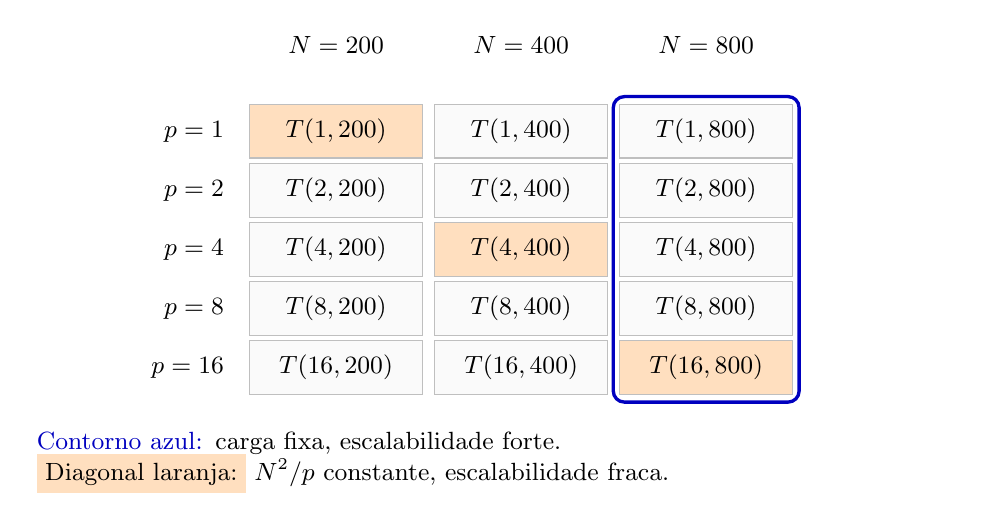
\begin{tikzpicture}[font=\small]
\foreach \n [count=\c from 0] in {200,400,800}
  \node at (2.35*\c+1.1,.75) {$N=\n$};
\foreach \p [count=\r from 0] in {1,2,4,8,16}{
  \node[anchor=east] at (-.2,-.75*\r-.35) {$p=\p$};
  \foreach \n [count=\c from 0] in {200,400,800}{
    \fill[gray!4] (2.35*\c,-.75*\r) rectangle ++(2.2,-.68);
    \ifnum\p=1 \ifnum\c=0 \fill[orange!25] (2.35*\c,-.75*\r) rectangle ++(2.2,-.68);\fi\fi
    \ifnum\p=4 \ifnum\c=1 \fill[orange!25] (2.35*\c,-.75*\r) rectangle ++(2.2,-.68);\fi\fi
    \ifnum\p=16 \ifnum\c=2 \fill[orange!25] (2.35*\c,-.75*\r) rectangle ++(2.2,-.68);\fi\fi
    \draw[gray!50] (2.35*\c,-.75*\r) rectangle ++(2.2,-.68);
    \node at (2.35*\c+1.1,-.75*\r-.34) {$T(\p,\n)$};
  }
}
\draw[blue!75!black,very thick,rounded corners]
(4.62,.1) rectangle (6.98,-3.78);
\node[align=left,text width=11.8cm] at (3.2,-4.55)
{\textcolor{blue!75!black}{Contorno azul:} carga fixa, escalabilidade forte.\\
\colorbox{orange!25}{Diagonal laranja:} $N^2/p$ constante, escalabilidade fraca.};
\end{tikzpicture}
\caption{Cada versão produz uma matriz de tempos. A coluna fixa compara equipes na mesma malha; a diagonal compara $200^2/1=400^2/4=800^2/16$ células por thread.}
\label{fig:matriz}
\end{figure}
